\documentclass[Lau,oneside]{sapthesis}%remove "english" for a thesis written in Italian
%Bachelor's (laurea triennale) thesis : Lau
\usepackage[english]{babel} %use this package for a thesis written in Italian
\usepackage[utf8]{inputenx}
\usepackage{indentfirst}
\usepackage{microtype}
\usepackage{amsmath}
\usepackage{amssymb}
\usepackage{float}
\usepackage{titlesec}
\usepackage{lettrine}
\usepackage{caption}
\usepackage{subcaption}
\usepackage{listings}
\usepackage[toc,page]{appendix}
\linespread{0.9}
\usepackage[nottoc, notlof, notlot]{tocbibind}
%\onehalfspacing
%\counterwithout{footnote}{chapter}
\usepackage{hyperref}
\hypersetup{		
			colorlinks=true,
			linkcolor=red,
                        linktoc=page,
			anchorcolor=black,
			citecolor=red,
			urlcolor=blue,
			pdftitle={Analysis of fuzz testing campaigns (temp)},
			pdfauthor={Matteo Sabatini},
			pdfkeywords={thesis, sapienza, roma, university}
}

\title{Analysis of fuzz testing campaigns (temp)}
\author{Matteo Sabatini}
\IDnumber{1794627}
\course{Cybersecurity}
\courseorganizer{Facolt\`a di Ingegneria dell'informazione, informatica e statistica}
\submitdate{2023/2024}
\copyyear{2024}
\advisor{(Prof. ??) Daniele Cono D'Elia}
\coadvisor{???}
\authoremail{sabatini.1794627@studenti.uniroma1.it}
\examdate{(??)}
\examiner{Prof. ??} \examiner{Prof. ??} \examiner{Prof. ??}  \examiner{Prof. ??}  \examiner{Prof. ??} \examiner{Prof. ??}  \examiner{Prof. ??}
\thesistype{Master thesis}

%we refer to http://ctan.mirrorcatalogs.com/macros/latex/contrib/sapthesis/sapthesis-doc.pdf for an exhaustive description of the sapthesis documentclass.






\begin{document}


\setlength{\parindent}{0pt}    %elimina l'indentazione leggermente a destra per ogni nuovo capitolo/paragrafo
\frontmatter
\maketitle

\begin{acknowledgments}
non so mai che scriverci :(
\end{acknowledgments}


\begin{abstract}
???
\newline \newline
\end{abstract}




\tableofcontents


\titleformat{\chapter}[display]  
{\normalfont\Huge\bfseries}{\chaptertitlename\ \thechapter}{20pt}{\huge}  
\titlespacing{\chapter}{0pt}{0pt}{0pt}  

\mainmatter
\chapter{Introduction}
\ \\
What is fuzz testing, how it works and why it is important...
\newline \newline
Brief explanation of the pros and cons of fuzzing...
\newline \newline
Google providing ways to fuzz your open-source software...
\newline \ \\
Objective of the thesis...
\newline \ \\
Main work done...
\newline \ \\
Brief summary of how the thesis is structured...




\chapter{Background}
\ \\
In the context of software development, \textit{fuzz testing} (or \textit{fuzzing}) refers to an automated software technique which focuses on providing random data to a program, with the objective of creating invalid or unexpected inputs that may potentially trigger crashes, assertions or memory leaks.
\newline 
This also allows developers to test their programs for so called "corner-cases", meaning situations that are hard or complex to reproduce as they should not occur when the program is being properly used, but still that could lead to unexpected and/or potential malicious behavior and thus should be properly handled. 
\newline \newline
Most fuzzers take structured inputs as reference, that will be used to generate inputs that are "valid enough" to be accepted by the program, but the strategies applied to generate such new inputs can heavily influence the effectiveness of the tests as well as the code-coverage achieved.
\newline
For this reason, fuzzers can be categorized using the 3 following characteristics:
\begin{itemize}
    \item how new inputs are generated (\textit{generation-based} or \textit{mutation-based})
    \item whether they are aware of the input structure (\textit{smart fuzzers}) or not (\textit{dumb fuzzers})
    \item whether they are aware of the program structure (\textit{white-box}), partially aware (\textit{gray-box}) or not (\textit{black-box})
\end{itemize}
It's important to mention that there is a trade-off between results, time spent testing and resources available.
\newline
Fuzzing is a technique that is quite resource-intensive, putting the CPU cores under heavy load while also generating potentially enormous log files, and these tests are usually run for several hours or even days, but preparing the right set of inputs that will be used to perform the tests is crucial to obtain good results.
\newline
Moreover, during a fuzzing session, there will be a point in time where either the inputs generated by the fuzzer will not trigger new execution flows or no new bugs are discovered for quite some time: reaching this state does not mean that the program is finally free of other bugs, as the conditions to trigger them might simply have not happened yet, and it's obviously impossible to know when this will happen as bugs may be discovered randomly.
\newline \newline \newline
Among the many results achieved thanks to this technique, two honorable mentions can be linked to the popular fuzzer \textit{American Fuzzy Lop} (also known as \textit{AFL} \cite{ref:AFL}).
\newline
In September 2014, AFL was used to discover "Shellshock" \cite{ref:shellshock} (also known as "Bashdoor"), a family of security bugs that affected the Unix Bash shell allowing malicious users to execute arbitrary commands without confirmation.
\newline
In April 2015, AFL discovered the famous "Heartbleed" \cite{ref:heartbleed} bug in OpenSSL, which allowed malicious users to decipher the otherwise encrypted communication from the TLS protocol. 
\newline \newline
This thesis will focus on two campaigns maintained by Google called \textit{OSS-Fuzz} \cite{ref:doc-ossfuzz} and \textit{FuzzBench} \cite{{ref:doc-fuzzbench}}: the first is a free platform that allows open-source developers to fuzz their programs autonomously relying on the computing resources provided by the Google Cloud service, while the latter allows fuzzer developers to test and improve their tools on real-word benchmarks thanks to automated tests and periodic reports.
\newline \newline
More specifically, it revolves around fuzzing some of the projects that have been implemented in these repositories using alternative approaches, trying to discover new and relevant bugs that will be then securely reported and disclosed to their developers in hope to have them fixed.

\newpage
\section{What is Fuzz Testing}
As previously mentioned, \textit{fuzz testing} is a software testing technique that feeds invalid, random and unexpected data to a program with the objective of discovering inputs whose execution may lead to crashes, failing assertions and memory leaks.
\newline \newline
We mainly distinguish between 3 types of fuzz testing:
\begin{itemize}
    \item \textbf{application fuzzing:} used for UI elements (such as buttons, input fields) or command-line programs, tests may include high-frequency inputs, providing random/invalid content and inputs exceeding the expected size
    \item \textbf{protocol fuzzing:} used to test the behavior of network elements and servers when invalid messages are sent over a chosen protocol, useful to ensure that such content is not misinterpreted and potentially executed as commands
    \item  \textbf{file format fuzzing:} used for programs that accept "structured inputs", meaning files that have a precise and standard format (like .doc, .jpg) which the fuzzer can modify with the intention of triggering unwanted behavior
\end{itemize}
This work will focus on testing programs that accept input files to provide their services, and for this reason several corpora were used to instruct the fuzzer on the appropriate file format. This will be discussed more in depth in section \ref{fuzzers}.
\newline \newline
One of the main requirements in fuzz testing is to achieve a high degree of \textbf{code coverage}: this statistic measures the percentage of source code executed in a test session, therefore achieving a high value means lowering the chance of leaving parts of the program with undetected bugs. Given this, one could argue that the fuzzer should be aware of the program's structure to maximize the coverage, but given that this process requires a non-trivial overhead it comes with its own trade-offs.
\newline \newline
For this reason, we define 3 different approaches.
\newline \newline
The \textit{black-box testing} involves using a fuzzer that is completely unaware of the program's structure, therefore assumes the program as a simple machine that takes a random input and generates an according output. This approach is relatively fast, can be easily parallelized and has good scalability. On the other hand, it will most likely find only "surface" bugs, i.e. they do not require particular conditions to be met to be triggered.     
\newline \newline
The \textit{white-box testing} involves using a fuzzer that employs "program analysis" techniques to systematically explore and reach critical program locations through meticulously crafted inputs, allowing you to discover bugs that could be potentially hidden deep in the program, although heavily relying on this knowledge implies that bugs related to unknown aspects of the program can be easily missed. While this approach is arguably the most effective one, the time used to analyze the program as well as generating such specialized input exponentially increases with the program complexity.
\newline \newline
The \textit{gray-box testing} attempts to integrate the best aspects of both approaches: use a minimal amount of knowledge over the program's structure to achieve a sufficient degree of code coverage such that the results obtained are satisfactory. This is usually done thanks to "instrumentation", discussed in section \ref{sanitizers}.
The previously mentioned AFL, which has been extensively used in this work, falls in this category.

\newpage
A fuzzing session usually yields two outputs: a set of "interesting" inputs and a list of potential bugs.
\newline \newline
Whenever a generated input results in a new execution flow, it is saved along with others "interesting inputs", which can be used in subsequent fuzzing sessions to provide the fuzzer with even more information about the structure of a good input that explores the deepest parts of the program. Then, the developer might decide to analyze and group these lists, to create a new one that does not contain duplicates and/or inputs triggering the same execution flows, which is particularly useful to ensure that the size does not explode over time.
\newline \newline
Regarding the discovering of bugs, a fuzzer has to be sensible enough to distinguish between crashing and non-crashing inputs without having full knowledge over the program tested, and "sanitizers" are used to inject assertions that make the program crash when a particular kind of failure is detected. Section \ref{sanitizers} explains this concept more thoroughly.
\newline
Then, the fuzzer might produce one (or more) inputs that triggered different kind of bugs, and the developer has to perform what is called \textit{bug triage}:
\begin{itemize}
    \item execute each input individually and observe the output
    \item determine which kind of error occurred and why, maybe also introducing debugging tools
    \item fix the bug entirely, if possible, or at least patch the problem as much as possible
    \item ensure that the bug does not occur in future fuzzing sessions by including the triggering input(s) in the set used for the tests
\end{itemize}
\ \\
Finally, it's important to recall that running a fuzzing session for several days or weeks without bugs does not necessarily imply that the program is secure: this process is driven by randomness, initial inputs provided and environment used, meaning also that each fuzzing session will always result in slightly different results and coverage achieved. Yet, testing a program on all possible inputs is obviously impossible.
\newline
Moreover, it easily generates false positives (trivial or benign warnings) and false negative results (incorrect or misleading results), further overloading the already tedious work of manually assessing each bug.

\ \\ \newline \newline
\newline \newline
Explain the main shortcomings of fuzz testing (maybe also available solution to mitigate them???)...



\newpage
\section{Different types of Fuzz Testers} \label{fuzzers}
A fuzzer is composed by the following key elements. \cite{ref:afl_docs}
\newline \newline
\textbf{Observer.}\ \ \ Provides information observed during the execution of a program to the fuzzer. Such information may be relatively simple, like the total running time for a single test and its output, to more advanced ones, like the maximum depth of the stack in a single execution. They are usually not preserved across many execution, unless an "interesting input" is encountered, in which case they are relayed to other nodes to improve future fuzzing sessions. 
\newline \newline
\textbf{Executor.}\ \ \ Responsible for defining how the program will be executed and the arguments passed on each run. The input for a single test is provided either by writing it in some specific memory location or passed as argument to a so called "harness function", although each fuzzer has its own implementation of this element. Given this, we briefly mention few standard functionalities that compose this element. The \textit{InProcessExecutor} runs the "harness function" and provides crash detection. The \textit{ForkServerExecutor} is responsible for spawning different child processes to fuzz. The \textit{TimeoutExecutor} wraps and installs a timeout for another running executor.
\newline \newline
\textbf{Feedback.}\ \ \ Classifies the result of a single execution and determines if the initial input is "interesting" or not, which is usually determined by retrieving information for the observers and analyzing the updated coverage map. It's also possible to define several of these elements, each one with its own objective (crashes, timeout, new execution flow discovered), and combine them in boolean expression to collect more fine-grained results.
\newline \newline
\textbf{Input.}\ \ \ Data taken from an external source and provided to the tested program to observe its behavior, usually in the form of bytes arrays. The first fuzzing session takes a set of inputs that is defined and provided by the developer itself, while future fuzzing session will also rely on previously discovered "interesting inputs". 
\newline \newline
\textbf{Testcase.}\ \ \ Defined as an input and a set of related metadata, like ID, description and expected results.
\newline \newline
\textbf{Corpus.}\ \ \ Location where testcases are stored, usually disk or memory. An example of input corpus may be composed by several testcases with the same properties, like crashing the program under a specific situation. An example of output corpus may be composed by all the testcases that are considered "interesting".
\newline \newline \newline
This thesis focused on using fuzzers capable of generating new structured inputs for the tested program starting from an initial \textit{seed}, specifically files with a precise format, allowing them to distinguish between a valid and an invalid example. 
\newline
However, even files that do not necessarily follow the defined structure can still be used as input for fuzzing, maybe with an even higher chance of triggering unwanted or unexpected behavior: for this reason, an effective fuzzer should be capable of generating inputs that are "valid enough" so that they are not rejected from the program's parser, and "invalid enough" to potentially trigger corner cases.


\newpage
We finally define the two main types of fuzzers.
\newline \newline
The \textbf{mutational-based fuzzers} require a corpus of seed inputs as reference, and generate new inputs by applying "mutators" on the provided seeds: these operations range from flipping single bits or bytes on a given input or performing mathematical operations over them, to adding or removing said information, sometimes even completely randomizing its content. Furthermore, these mutation may be mixed-and-matched into long sequences, to generate even more new inputs.
\newline
A \textit{smart mutational fuzzer} might leverage its knowledge on the input model to switch between different types of inputs, although this information is not always available.
\newline
A \textit{dumb mutational fuzzer}, like AFL, employs random mutations using as reference the content of "interesting inputs", which usually results in a much lower proportion of valid inputs generated.
\newline \newline
The \textbf{generation-based fuzzers} generate new inputs from scratch, usually relying on a good source of randomness to perform this operation, and for this reason they do not depend on the existence of a good corpus nor its quality.
\newline
A \textit{smart generation fuzzer} might leverage the input model provided by the developer to generate valid new inputs, although this information may not always be available.
\newline
A \textit{dumb generation fuzzer} attempts to generate new inputs without any reference, oftentimes putting more stress on the program's parser rather than the program itself, as they generate an overwhelmingly amount of invalid inputs.







\newpage
\section{Open-Source Software}
The \textbf{Open-Source Software (OSS)} is a computer software developed in a collaborative and public manner, released under a particular license that allows other users to freely use, study, modify and distribute the software and its source code for any purpose: this allows many users to actively participate in the development of a software by proposing changes and new improvements.
\newline \newline
To be eligible as an open-source software, the license's distribution terms must comply with the following criteria: \cite{ref:osd}
\begin{enumerate}
    
    \item \textbf{Free redistribution} \newline 
    The license must not restrict anyone from selling or giving away the software as part of a suite, nor it could be used to require royalties or fees on such sales.
    
    \item \textbf{Source code} \newline
    The program must include its source code, provided in a form that allows other programmers to modify it, as well as a compiled version. If the source code cannot be distributed, it should be easily obtainable thanks to well-publicized means, ideally downloadable from the Internet free of charge.
    It is not allowed to provide obfuscated source code or any partially-compiled form.
    
    \item \textbf{Derived works} \newline
    The license must allow for modifications and publishing of derived works, allowing them to be distributed under the same license of the original software
    
    \item \textbf{Integrity of the author's source code} \newline
    If the developers want to protect the original source code, they must allow the distribution of "patch files" to perform modification of the program at compile time. In this case, the license must explicitly allow distribution of software built from a modified source code as long as any derived works carry a different name or version number with respect to the original software. 
    
    \item \textbf{No discrimination against person or groups} \newline
    The license must not discriminate against any person or group of persons.
    
    \item \textbf{No discrimination against fields of endeavor} \newline
    The license must not restrict anyone from using the program in a particular field of endeavor or work.
    
    \item \textbf{Distribution of license} \newline
    The license's rights provided must apply for anyone that obtains the product, whether it is the original software or a redistributed version of it.
    
    \item \textbf{License must no be specific to a product} \newline
    The license's rights must not depend on the program being part of a suite. If that is true, the license of such suite must follow the same rights as those granted with the original software distribution. 
    
    \item \textbf{License must not restrict other software} \newline
    The license must not put restrictions of any other software that might be distributed along with the licensed software.
    
    \item \textbf{License must be technology-neutral} \newline
    No license provision may be linked to a particular technology or interface style.
\end{enumerate}
There are some key points that should be considered during the development of open-source software.
\newline \newline
First, the authors must decide how the program will be developed.
\newline
Usually, this software is released under two development branches: a "stable" version, composed by all the functionalities that have been thoroughly tested and work as intended, and a "build" version, that is slightly buggier as it includes proposed changes and new features that have yet to be refined.
Releasing the "build" version early not only allows the developers to showcase their work and attract even more new users, but also provides them with feedback from real users that are willing to run untested versions of their software.
\newline \newline
Then, they must decide how they will interact with online users.
\newline
In this sense, providing full access to the source code means that other users can submit new additions to the software, bug reports and code fixes as well as point out mistakes in the documentation, therefore helping the original developers in their works while also improving and refining the product. Moreover, given that each user may have different knowledge and programming skills as well as different testing environments, this allows to test and benchmark the product on a wide range of systems further increasing the probabilities of finding new and unknown bugs that may be specific to a single OS or architecture.
\newline \newline
Finally, it is important to mention that although any user has the rights to mention a bug, error, or mistake in the program, it is still up to the developers to ensure the truthfulness of what has been reported and how to tackle it.
\newline
For example, bugs that are not security-relevant or that may be related to QoL aspects are easily pushed back as secondary problems or simply ignored altogether.
Sometimes, if the developer are kind enough to accept your request but do not have time and resources to solve it, they might ask the user themselves for a proposed fix and cite them in the next patch notes as a way of thanking them.
\newline \newline
As will be discussed in future sections, while many reports produced in this work highlighted several security bugs that have been fixed in short times, some have been ignored due to them being not relevant at the moment of reporting or because they were declared as an incorrect building approach and/or use of the program itself.   
\newline \newline \newline
Given all this, one could argue that providing complete access to the source code and allowing other people to suggest changes poses a real threat to the security of the program.
\newline
History has shown us many times that, given enough time and resources, releasing the source code of a program will result in malicious users discovering bugs and vulnerabilities that could have potentially catastrophic consequences. Moreover, a malicious user might try to suggest a modification in the code that introduces a specific vulnerability or generate a bug report containing false information with attachments that might exploit a previously unknown vulnerability.
\newline
This is why having a large users base is important and one of the main advantages of open-source: if many people are closely watching how the program is being developed, one of them will most likely realize that malicious modifications are being suggested and notify others of the situation.
\newline \newline
Few noticeable mentions (LibreOffice, VLC, Firefox, etc...) ???




\newpage
\section{Fuzzing with Google}
The \textit{Google Open Source Project} \cite{ref:google_oss} is a campaign started in 2004, one of the oldest open-source campaigns in the industry. 
\newline
It was initially meant to share Google-developed software under open licenses, with the intention of bringing free technology and information sharing to the public, but it quickly became a program dedicated to improving open-source ecosystems as a whole. 
\newline \newline
Thanks to this campaign, many projects became popular and gained worldwide recognition such as Android OS, TensorFlow, the Go programming language, and many more.


\ \\
\subsection{OSS-Fuzz}
The \textit{OSS-Fuzz Project} was created in 2016 after the famous "Heartbleed" vulnerability was discovered in OpenSSl, one of the most popular open-source projects at the time for encrypting web traffic, as a response to provide developers with free fuzzing and private alerts services for their open-source projects.
While it was initially intended for languages that are not memory-safe (C/C++), it is now capable to provide support for other popular languages such as Python, Go, Java and Rust.  
\newline
As of August 2023, it helped identify and fix over 10.000 vulnerabilities and 36.000 bugs across over 1000 projects. \cite{ref:ossfuzz_docs}.
\newline \newline
Projects can be tested using several fuzzing engines (such as LibFuzzer, AFL++, Honggfuzz and Centipede) in combination with Google Sanitizers (ASan, MSan and UBSan), while \textit{ClusterFuzz} acts as the back-end and reporting tool.
\newline \newline
\begin{figure}[h]
\makebox[\textwidth][c]{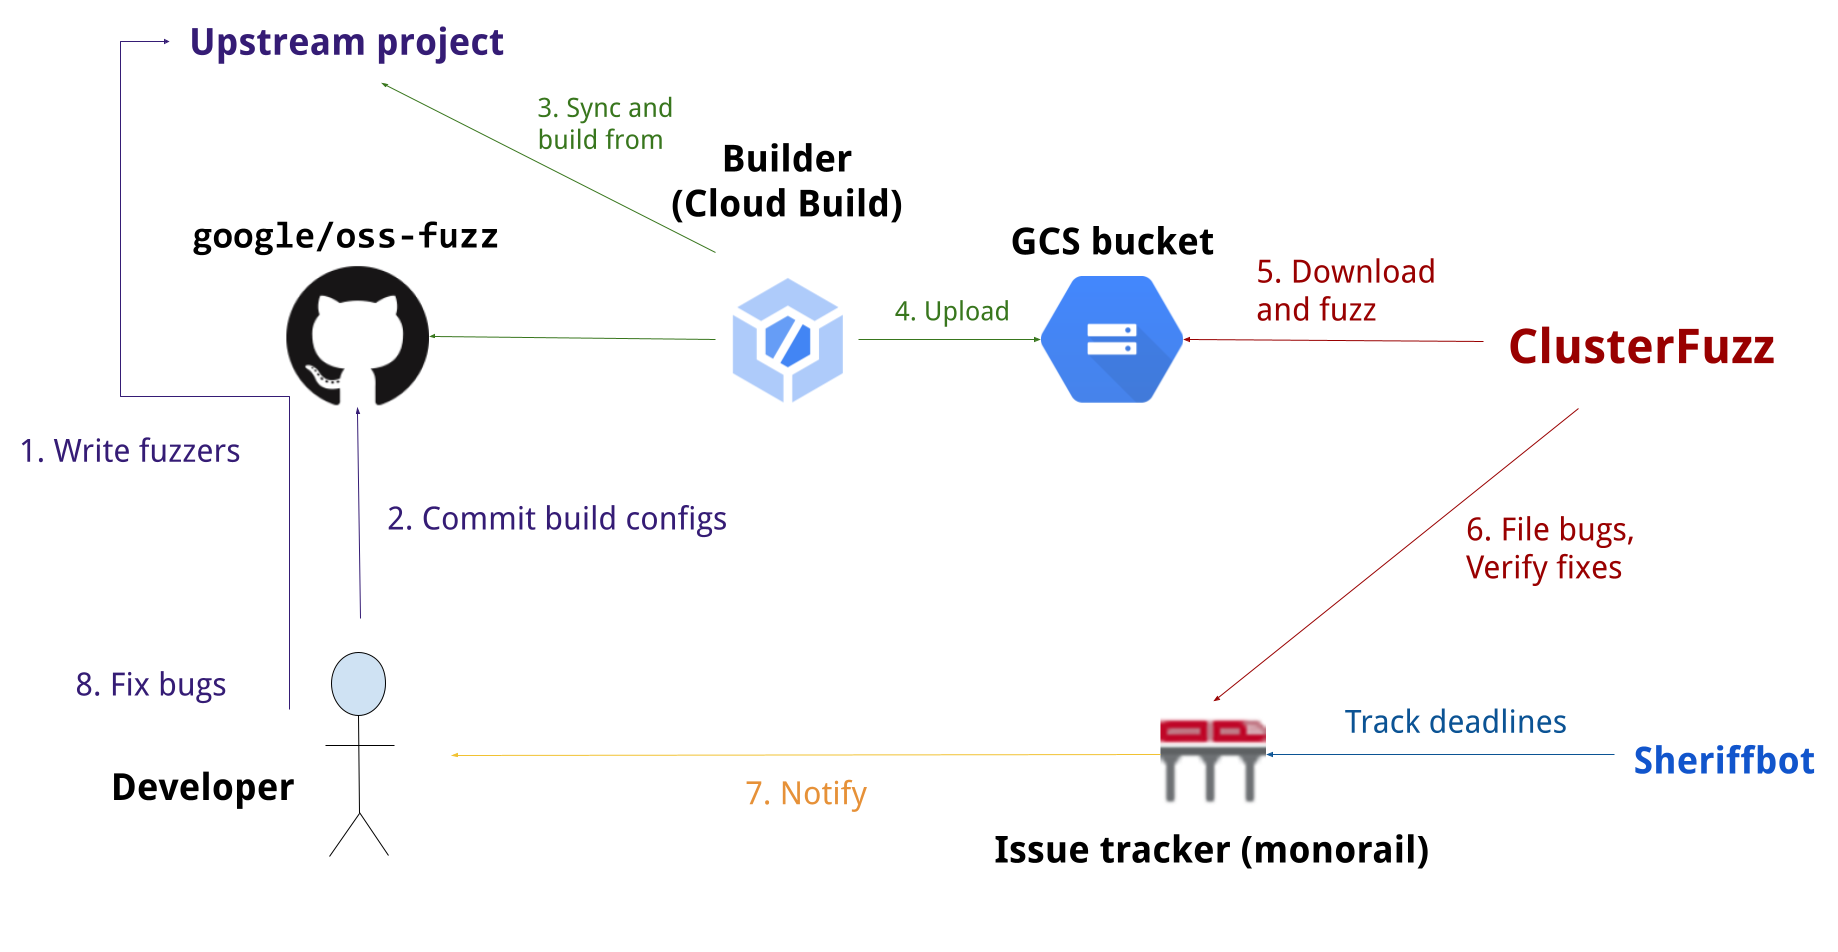
\includegraphics[width=0.77\paperwidth]{foto/oss-fuzz_architecture.png}}
\caption{OSS-Fuzz main architecture visualized \cite{ref:ossfuzz_docs}}
\label{fig:ossfuzz_architecture}
\end{figure}

\newpage
The process works as follows.
\newline \newline \newline
Initially, the maintainer of an open-source project creates one or more "fuzz targets" that will be integrated with the project's build and test systems. \cite{ref:libfuzzer_docs}
\newline
A "fuzz target" is essentially a function that accepts an input, in this case an array of bytes, and perform some operations with these bytes to test a specific API.
\newline
Although not all projects are expected to implement and maintain their targets in the same way, developers can refer to a guide of recommendations to increase the efficiency and quality of the automated fuzzing tests performed.
\newline
To briefly summarize them, they should:
\begin{itemize}
    \item maintain the source code and targets' build system using some versioning service (like Git)
    \item allow each fuzz target to be compiled with Sanitizers
    \item avoid modular build systems for the fuzz targets (compile all or nothing) and use general-scope compile flags
    \item provide a seed corpus that is regularly updated and extended with new "interesting inputs", also it should have good coverage
    \item provide a dictionary of tokens to instruct the fuzzer on the correct syntax of the inputs, if applicable
    \item periodically check the performances achieved by each fuzz target, meaning their coverage, time spent on execution and solving abrupt errors
\end{itemize}
\ \\
Then, the newly prepared project must be accepted by OSS-Fuzz, which is done by issuing a "pull request" on the project repository with some requested information, such as: project's main repo, language used, building instructions and email addresses to contact on new issues.
\newline
On the other end, a bot periodically checks for new requests and validates their content before accepting/rejecting them.
\newline \newline \newline
Once the project has been accepted as part of the OSS-Fuzz's infrastructure, a "builder" script follows the provided instructions to build the project's fuzz targets and uploads them to a Google Cloud Service Bucket, a file-hosting service.
\newline
This acts as a middle point between OSS-Fuzz and ClusterFuzz, which uses the aforementioned bucket to download all the necessary elements to fuzz the project as well as upload the results achieved.
\newline \newline \newline
After a successful fuzzing session, any bug discovered is reported to the OSS-Fuzz issue tracker \cite{ref:ossfuzz_bugtracker}, which uses the metadata sent by ClusterFuzz to automatically create a report. 
\newline
Developers have 3 ways of dealing with this situation: they can commit new changes to fix the bug (verified by ClusterFuzz before closing an issue), assign the tag "WontFix" to the bug to notify that it will not be solved, or simply ignore it altoghether. 
\newline \newline
These steps create a cycle that allows for continuous fuzzing and improvement of the software.


\newpage
Finally, OSS-Fuzz follows a strict \textit{bug disclosure guideline}. \cite{ref:bug_disclosure}
\newline \newline
When a bug is discovered, an automatic email is generated and sent to all email addresses specified in the project, and an issue is opened on the issue tracker.
\newline
This email contains the report created using ClusterFuzz, as well as an estimation of the priority and severity of the bug discovered.
\newline \newline
From this moment, the issue will be publicly visible in 90 days or after the fix is released (whichever comes earlier), meaning that anyone will have access to the causing input as well as any other debugging information related to what happened and how to reproduce the bug.
\newline
Before the deadline expires, the developers may request a 14-day grace period if the patch is set to be released on a specific day within this extended period, in which case the public disclosure is delayed.
\newline \newline
In any case, Google reserves the right to change deadlines forwards or backwards depending on the circumstances and the severity of the findings.





\ \\
\subsection{ClusterFuzz}
The \textit{ClusterFuzz Project} is a scalable fuzzing infrastructure with the objective of discovering security and stability issues in software, it is the main platform used by Google to test its own products and also the fuzzing back-end for \textit{OSS-Fuzz}.
\newline
As of May 2023, it discovered over 25.000 bugs in Google proprietary software (e.g. Chrome) and 36.000 bugs with OSS-Fuzz. \cite{ref:clusterfuzz_docs}
\newline \newline
It is based on a highly scalable distributed system of VMs, performing fully automatic bug filing, triage and closing as well as performance reports.
\newline \newline
\begin{figure}[h]
\makebox[\textwidth][c]{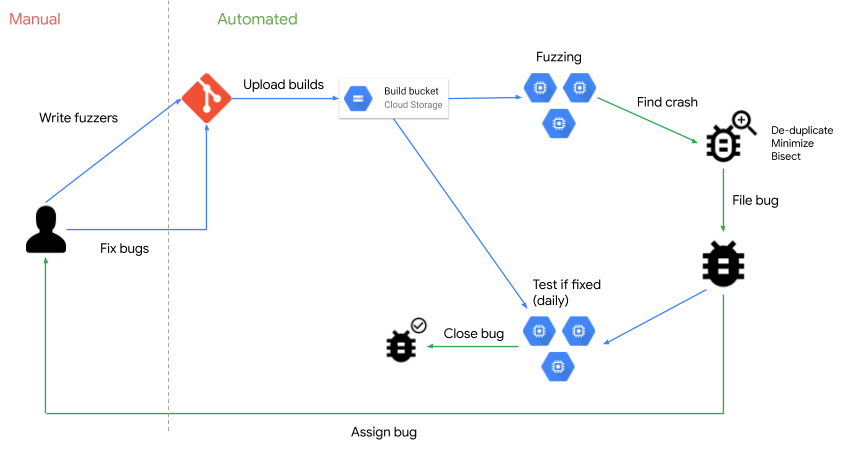
\includegraphics[width=0.665\paperwidth]{foto/clusterfuzz_architecture.png}}
\caption{ClusterFuzz main architecture visualized \cite{ref:clusterfuzz_docs}}
\label{fig:clusterfuzz_architecture}
\end{figure}
\ \\
All operations are performed by two components.
\newline \newline
The \textit{App Engine} provides a web interface to the information collected during each fuzzing session, allowing the developers to easily access crashes, results and other information. This is also where tests can be scheduled, which is done via \verb|cron| jobs.
\newline \newline
The \textit{Fuzzing Bots Pool} is a cluster of VMs responsible for running the scheduled fuzzing sessions, and they perform the following operations:
\begin{itemize}
    \item \textbf{fuzz:} runs a fuzzing session
    \item \textbf{progression:} checks if a testcase still reproduces or if has been fixed
    \item \textbf{regression:} calculates the revision range in which a crash was introduced
    \item \textbf{minimize:} eliminates duplicate testcases from the input seeds
    \item \textbf{pruning:} minimize a corpus to the smallest size based on coverage information
    \item \textbf{analyze:} runs a manually uploaded testcase against a specific job to see if it crashes
\end{itemize}
\ \\
Given that some of this tasks are critical and should be treated as atomic operations, bots can be \textit{preemptible} or \textit{non-preemptible}.
\newline
The first refers to a machine that can only run the "fuzz" task as it can be shut down at any moment.
\newline
The latter refers to a machine that is not expected to abruptly stop or crash, therefore is capable of running all tasks.
\newline \newline \newline
Each VMs performs these operations inside Docker instances, created and provided by the developer using Dockerfiles, that are configured with all the tools and files necessary to correctly build and launch the fuzzing targets.





\ \\
\subsection{FuzzBench}
The \textit{FuzzBench Project} is a free service that provides fuzzers' developers with several real-world benchmark tested at Google scale, comparing the results with other famous fuzzers (such as AFL and LibFuzzer) and allowing them to evaluate their performances thanks to daily reports for further improvements.
\cite{ref:fuzzbench_docs}
\newline
\begin{figure}[h]
\makebox[\textwidth][c]{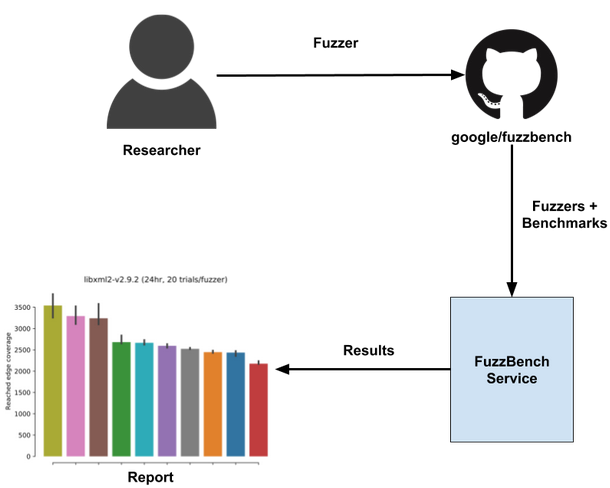
\includegraphics[width=0.67\paperwidth]{foto/fuzzbench_architecture.png}}
\caption{FuzzBench main architecture visualized \cite{ref:fuzzbench_docs}}
\label{fig:fuzzbench_architecture}
\end{figure}
\ \\
The process works as follows.
\newline \newline
Initially, a fuzzer developer integrates its product within FuzzBench using a Dockerfile, containing all the resources necessary to build targets using the fuzzer and where all benchmarks will be executed.
\newline
Similarly to OSS-Fuzz, this process is done via "pull requests", which are automatically revisioned and accepted by bots.
\newline \newline
Then, the developers may choose between two testing approaches: standard and OSS-Fuzz.
\newline
In the first case, the benchmark is created and defined by the developers themselves, and this requires the definition of fuzz targets, build files and Docker images that will be used to correctly build and link the fuzzer to the targets and run the tests.
\newline
In the latter, the developers employ a fuzz target from any OSS-Fuzz project as benchmark, allowing them to test their product on a real-world scenario.
\newline \newline
Finally, a report will be created highlighting the strengths and weaknesses of the fuzzer on the various benchmarks, comparing individual and overall results with other fuzzers.





\newpage
\chapter{Preliminary Work}
\ \\
\section{Understanding OSS-Fuzz projects}
To be accepted by OSS-Fuzz, the developers create a "pull request" to the OSS-Fuzz repository, but only projects that are relevant and/or critical to the global IT infrastructure with a significant user base will be integrated.
\newline \newline
To check if your project is eligible for OSS-Fuzz, Google provides a mathematical formula to calculate the "Open-Source Project Criticality Score" \cite{ref:score} in a range between 0 \textit{(least critical)} and 1 \textit{(most critical)}, which is the following:
\ \\
\begin{equation}
    CriticalityScore = \frac{1}{\sum \alpha_i}\  \sum_i \alpha_i \ \frac{\log(1+S_i)}{\log(1+\max(S_i,T_i))}
\end{equation}
\ \\
The parameters evaluated are the followings:
\begin{itemize}
    \item \textbf{created-since} ($\alpha_i = 1$, $T_i = 120$): months since the project was created
    \item \textbf{updated-since} ($\alpha_i = -1$, $T_i = 120$): months since the project was last updated
    \item \textbf{contributor-count} ($\alpha_i = 2$, $T_i = 5000$): count of commits made by distinct contributors
    \item \textbf{org-count} ($\alpha_i = 1$, $T_i = 10$): count of distinct organizations contributing to the project
    \item \textbf{commit-frequency} ($\alpha_i = 1$, $T_i = 1000$): average number of commits per week in the last year
    \item \textbf{recent-releases-count} ($\alpha_i = 0.5$, $T_i = 26$): number of releases in the last year
    \item \textbf{closed-issues-count} ($\alpha_i = 0.5$, $T_i = 5000$): number of issues closed in the last 90 days
    \item \textbf{updated-issues-count} ($\alpha_i = 0.5$, $T_i = 5000$): number of issues updated in the last 90 days
    \item \textbf{comment-frequency} ($\alpha_i = 1$, $T_i = 15$): average number of comments per issue in the last 90 days
    \item \textbf{dependents-count} ($\alpha_i = 2$, $T_i = 500000$): number of project mentions in the commit messages
\end{itemize}
\ \\
Only projects scoring a value $\geq 0.7$ may be eligible to be integrated in the OSS-Fuzz campaign.

\newpage
The main file structure of an OSS-Fuzz project is composed by 3 files.
\newline \newline
The \textit{project.yaml} configuration file stores project metadata needed by OSS-Fuzz to correctly provide its services, including:
\begin{itemize}
    \item \textbf{homepage:} url to the project's homepage
    \item \textbf{language:} programming language used to write the project (C, C++, Go, Rust, Python, JVM languages, Swift)
    \item \textbf{primary\_contacts:} list of email addresses that will be automatically CCed on crash reports and fuzzer statistics
    \item \textbf{main\_repo:} path to the source code repository hosting the project
    \item \textbf{vendor\_ccs:} \textit{optional}, list of vendors' email addresses that want access to the bug reports
    \item \textbf{sanitizers:} \textit{optional}, list of sanitizers that are available on the project (address, undefined, memory), if not specified "address" and "undefined" will be used
    \item \textbf{architectures:} \textit{optional}, list of architectures that can build the project (supported only x86\_64 and i386)
    \item \textbf{fuzzing\_engines:} \textit{optional}, list of fuzzing engines available (libfuzzer, afl, honggfuzz and centipede), if not specified "libfuzzer" will be used
    \item \textbf{help\_url:} \textit{optional}, used on reports to provide a custom guide related to bug reproduction steps
    \item \textbf{builds\_per\_day:} \textit{optional}, number of times a project should be built per day, OSS-Fuzz allows up to 4 builds per day and builds once per day by default
    \item \textbf{file\_github\_issue:} \textit{optional}, mirrors OSS-Fuzz bug reports on the project's GitHub repository via "Issues"
\end{itemize}
\ \\
The \textit{Dockerfile} defines a container with all the dependencies and resources needed to build the project and prepare the testing environment.
\newline
To avoid having developers create and maintain their own customized Docker containers and create an homogeneous and standard environment, OSS-Fuzz provides several "base images" for each supported language, built on top of Ubuntu 20.04 and with the appropriate compilers and toolchains already installed.
\newline
After pulling the most appropriate base image, there are usually several "apt-get" and "git clone" commands related to downloading and installing all the required packages and dependencies needed to correctly build the project.
\newline
Finally, the build script and any other fuzzer files are pulled from the project's repository.
\newline \newline
The \textit{build.sh:} script, executed inside the Docker container, performs all the operations necessary to build the project and the fuzzing targets that will be tested.
\newline
In general, the script should build the project and the fuzz targets using the correct compiler and appropriate compiler flags.
\newline
To provide a more flexible and accessible build system, the Docker image provides several environment variables regarding directory locations, compilers and compiling flags, allowing developers to easily retarget scripts with little effort.




\newpage
\section{Understanding FuzzBench benchmarks}
Explain what is a project in FuzzBench...
\newline \newline
Explain the structure of a project and its files...
\newline \newline
Explain the commands from the "gsutil" suite...




\newpage
\section{Sanitizers} \label{sanitizers}
A \textit{code sanitizer} is a tool used to detect bugs in a program during both compilation and runtime, and this is done by "instrumenting" the code.
\newline
The act of "instrumentation" refers to modifying either the source code or binary code that is being compiled to add some additional functionalities and references that can be used by other tools to perform code analysis, logging or profiling.
\newline
It's important to notice that this process is not only severely limited by the single execution flow analyzed, but also introduces a non-trivial overhead both in terms of increased execution time and memory usage, which may cause problems when it comes to managing computing resources.
\newline \newline
Although code sanitizers should be a standard practice in the development cycle of a program, unfortunately this is not the case as introducing these tools not only requires extensive tests to check for potential errors, but also because they do not always interact very well with shared libraries or other external dependencies.
\newline
It is also extremely important to mention that these bug detection tools are not meant to be linked against production executables, as their runtime was not developed with security-sensitive constraints and may compromise the security of the released product. \cite{ref:asan_docs}\cite{ref:msan_docs}\cite{ref:ubsan_docs}
\newline \newline
In this thesis, we focused on using several sanitizers developed by Google \cite{ref:san_repo} as part of its tools available to open-source developers to improve their programs and make them more secure, which proved to be particularly effective when combined with fuzzing due to its ability to trigger bugs.


\ \\
\subsection{ASan and LSan}
The \textit{Address Sanitizer} \cite{ref:asan_paper} is a memory error detection tool for C/C++ that helps developers to find and fix any out-of-bounds accesses to heap, stack and global objects as well as use-after-free bugs, and its one of the most widely used and effective sanitizers.
\newline \newline
It works by using a shadow memory to map the memory regions allocated by the application and record whether each byte of such areas can be safely accessed by load/store operations. Each memory region is assigned a shadow counterpart, containing metadata about its size and the offset range that can be used to safely access it, while any attempt to read/write beyond such boundaries will trigger a sanitizer error, as shown by the figure below:
\newline
\begin{figure}[h]
\centering
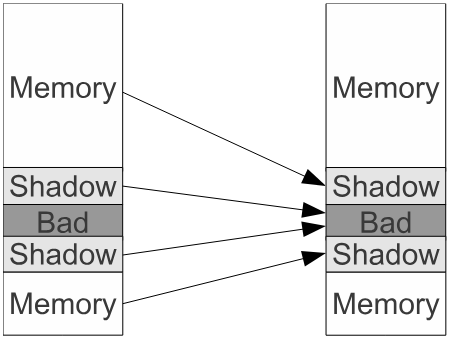
\includegraphics[scale=0.4]{foto/shadow_memory.png}
\caption{Memory mapping of ASan \cite{ref:asan_paper}}
\label{fig:asan_shadow}
\end{figure}
\newline
Detection of out-of-bounds accesses to globals and stack objects is done in a similar way, which means by creating poisoned memory regions around such objects: \textit{global variables} are poisoned at compile-time and their addresses computed during the application startup, while \textit{stack objects} are poisoned and recorded at run-time.
\newline \newline
The management of the shadow memory is done by ASan run-time library, containing specialized implementation of the \verb|malloc| and \verb|free| functions, which allocate extra memory for shadow and poisoned memory zones as well as keeping a FIFO stack of allocated and freed memory regions to detect use-after-free, double-free and invalid-free bugs.
\newline \newline
Finally, ASan adds a slight overhead, increasing execution times by an average 170\% and memory usage by 3.4x.
\newline \newline \newline
Another component is the \textit{Leak Sanitizer} (or \textit{LSan}), a memory leak detector enabled by default in ASan that returns which portions of the program are leaking memory as well as the size leaked, thanks to comprehensive and exhaustive stack traces. Although this tool may seem very helpful, it usually generate huge logs especially when having complex programs that heavily rely on external libraries, which oftentimes do not perform clean releases of the objects used.


\ \\
\subsection{MSan}
The \textit{Memory Sanitizer} \cite{ref:msan_paper} is a memory reads detector for C/C++ that helps developers to find and fix use-of-uninitialized-memory (UUM) bugs.
The C and C++ languages usually create uninitialized stack and heap objects (unless \verb|calloc| is invoked), and discovering these bugs can be quite tricky as they do not necessarily occur in every execution and could be triggered by any operation performed by the program.
\newline \newline
It works by using a shadow memory to map each bit of application memory and encode its state (0 initialized, 1 otherwise): all newly allocated memory is poisoned, i.e. the corresponding shadow memory is initialized to \verb|0xFF|, and "shadow propagation" operations are performed to safely copy an uninitialized variable between memory regions as well as simple logic and arithmetic operations without occurring in errors.
\newline
Performing a load operation from uninitialized memory returns an \textit{undefined value}, and operations like conditional branch, syscall and pointer dereference are most likely to trigger UUM bugs.
\newline
\begin{figure}[h]
\centering
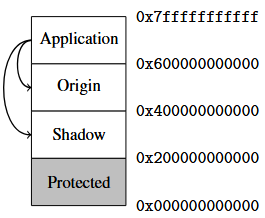
\includegraphics[scale=0.63]{foto/shadow_memory_2.png}
\caption{Memory mapping of MSan \cite{ref:msan_paper}}
\label{fig:msan_shadow}
\end{figure}
\newline
Given that UUM bugs are notoriously hard to reproduce and debug, the "origin-tracking-mode" can be used to obtain more comprehensive stack-traces and helping the developer to understand where it should have happened, although it relies on the program's symbols to provide meaningful information.
\newline
If necessary, there is also an "advanced-origin-tracking-mode", printing the stack traces of all operations from the allocation of the uninitialized variable up to its load, but its usability is still discussed due to the huge amount of memory it requires.
\newline \newline
The management of the shadow memory is done by MSan run-time library, that maps the "shadow" and (optional) "origin" areas and marks as uninitialized any new allocated regions as well as the deallocated ones. To update the shadow region, a large subset of the standard \verb|libc| functions are intercepted.
\newline \newline
Fixing UUM bugs is generally a quick task, like initializing the memory region using appropriate functions or simply setting all bytes to 0, but many developers avoid this sanitizer due to the huge slowdown that it introduces.
\newline
In fact MSan adds a modest overhead, increasing execution times by an average 300\% and memory usage by 2x on short programs, values that rapidly worsen with complex programs and when "origin-tracking-mode" is enabled.


\ \\
\subsection{UBSan}
The \textit{Undefined Behavior Sanitizer} \cite{ref:ubsan_docs} is a fast undefined-behavior detector for C/C++, that helps developers to find and fix undefined-behavior (UB) bugs.
\newline
Common operations that may lead to undefined behaviors are: array subscription out of bounds, overflows/underflows originating from mathematical or logical operations, dereferenced, misagnlied or null pointers and conversion between data types.
\newline \newline
By default, due to its simplistic nature, the tool does not print stack-traces and uses a minimal run-time library. If needed, "print-stacktrace-mode" can be enabled to obtain more comprehensive results, although it relies on the program’s symbols to provide meaningful information.
\newline \newline
Finally, UBSan adds a trivial overhead, increasing execution times by an average 120\% and memory usage by 2x.






\newpage
\section{Setting up the environment}
All tests were performed on two separate machines, both equipped with personal installations of Ubuntu 22.04 LTS, already run-in and used.
\newline \newline \newline
Regarding tools for general purpose, I used Docker, Valgrind, Python 3, gsutil and Google Chrome.
\newline \newline
The \textit{Docker} application was needed to run the different containers needed by OSS-Fuzz to build the projects and run the tests.
\newline \newline
\textit{Valgrind} \cite{ref:valgrind} is an instrumentation framework to perform memory analysis, profiling and management during the execution of a program.
More specifically, it was used to perform memory analysis in projects built without sanitizers.
\newline \newline
The \textit{Python 3} language was used to create several scripts that I used to perform information scraping, reports analysis and bug deduplication.
It is also used by OSS-Fuzz to provide some functionalities, and this will be discussed later. 
\newline \newline
The \textit{gsutil} suite is a command-line tool provided by Google to access resources stored on Google Cloud Service from your local machine, and it was used to analyze the FuzzBench benchmarks and download other resources.
\newline \newline
Finally, \textit{Google Chrome} and its "development driver" were needed during the information scraping phase of this work, discussed in section \ref{selection}.
\newline \newline \newline
Regarding \textit{OSS-Fuzz}, most of the work was done on its GitHub repository, which I cloned locally on both machines.
\newline
To provide its services, OSS-Fuzz uses several python scripts that can be invoked via command-line using appropriate arguments. These commands can be used to update the projects' files and projects' images, build the project's image and its fuzzers but also download resources like corpora. 
\newline \newline \newline
Regarding \textit{FuzzBench} [...]










\chapter{Methodology}
\ \\
\section{OSS-Fuzz}
\subsection{Selecting the projects} \label{selection}
At the moment of writing, the OSS-Fuzz campaign includes over 1000 projects that are actively fuzzed and tested, but it would obviously be impossible to rebuild and test all of them locally also due to the language heterogeneity of such projects.
\newline
For this reason, this work focused solely on projects using the C/C++ language.
\newline
Then, to further narrow down the analysis, I identified 5 different categories of projects using the number of sanitizers used by the developers, keeping ASan as the reference due to its popularity and efficiency.
\newline
Finally, I ordered each set by "highest number of bugs issued" using the OSS-Fuzz bug tracker and tested these lists top-down until I had 5 projects for each category that were building and fuzzing correctly.
\ \\ \newline \newline
First step in this process was to extract the list of all projects written in C/C++, and this was done by performing a preliminary analysis of the \textit{project.yaml} configuration file present inside each project's directory.
\newline
\begin{figure}[h]
\centering
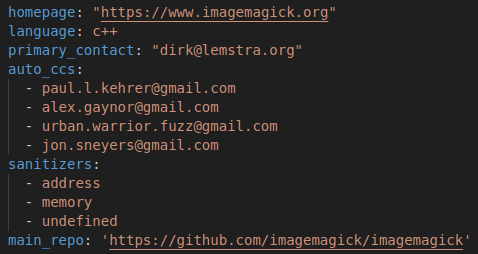
\includegraphics[scale=0.5]{foto/project_yaml.png}
\caption{Example of content from a project.yaml}
\label{fig:project_yaml}
\end{figure}
\ \\
To retrieve the language used by each project, I initially wrote a simple Python script taking as input the OSS-Fuzz "project" directory.
\newline
Then, the script retrieved the directory list of the argument provided and iteratively explored each project's directory looking for the aforementioned configuration file: assuming the file was found, it then opened the file and scanned each line looking for the "language: c" string, eventually saving the name of such projects in a list.
\newline \newline
This yielded a total of 524 projects out of 1277 written using C/C++.


\newpage
To perform the categorization of the projects depending on the number of sanitizers used, I extended the previous script to also look for the strings "address", "memory" and "undefined", shown on image \ref{fig:project_yaml}.
\newline
The assignment uses a binary logic on decimal values, starting each project from 0 and giving each sanitizer a different value (1, 10, 100), so that by summing them I could easily understand which sanitizers were found in its configuration file.
\newline \newline
Out of the previous 524 projects, the results were as follows: 238 used all sanitizers, 22 used ASan and MSan, 62 used ASan and UBSan, 46 used only ASan and 156 did not use any sanitizers.
\ \\ \newline \newline
The next step was retrieving the number of discovered bugs of each project, and this required a thorough analysis of the "OSS-Fuzz Issue Tracker" website. \cite{ref:ossfuzz_bugtracker}
\newline
\begin{figure}[h]
\makebox[\textwidth][c]{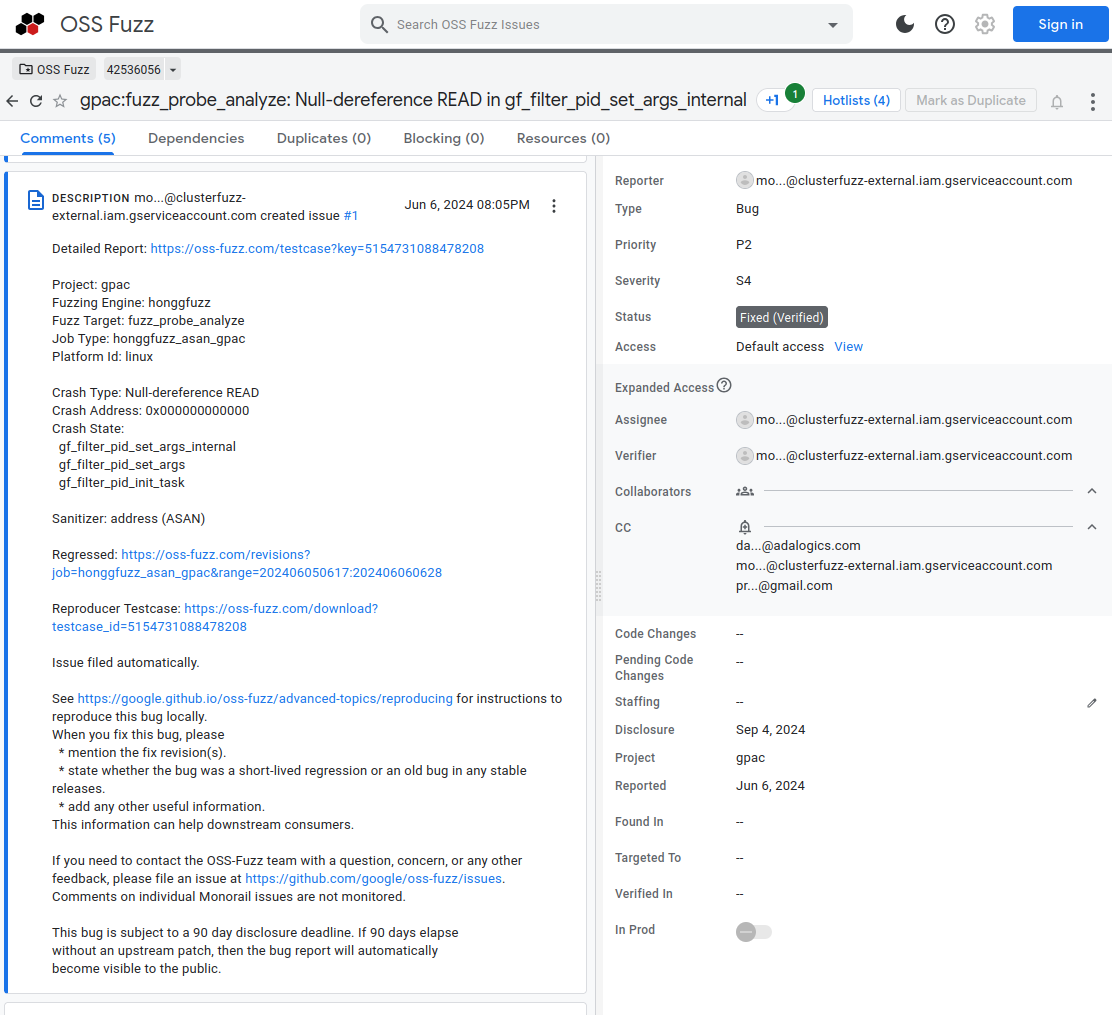
\includegraphics[width=0.69\paperwidth]{foto/issue.png}}
\caption{Example of bug report \cite{ref:ossfuzz_bugtracker}}
\label{fig:issue}
\end{figure}
\ \\
At the moment of writing, the issue tracker platform was changed from "Monorail" to "Google Sites", so most of the work described here may no longer work as intended.




\newpage
Given that Monorail APIs could only be used by projects' developers registered to OSS-Fuzz and that there weren't any files that could be used for an offline analysis, I had to perform website scraping on the individual issues to retrieve the information. 
\newline
To do this, I used as reference a GitHub repository written by Zhen Yu Ding called "Monorail Scraper" \cite{ref:scraper}, a tool to scrape and retrieve data from Monorail, that also included functionalities for ClusterFuzz-generated OSS-Fuzz issues.
\newline \newline
The tool relies on the Google Chrome web browser and their testing development tool called "ChromeDriver" \cite{ref:driver}: this is an autonomous web server implementing "W3C WebDriver" \cite{ref:driver_standard}, a standard providing a remote interface to control user-agents and a set of interfaces to perform analysis and manipulation of DOM elements.
\newline
Essentially, this allows the user to write scripts that, in turn, instruct the Google Chrome browser to visit a specific web page and possibly performs some interaction with it, like pushing a button, compiling a form or visiting another webpage by exploring the DOM elements.  
\newline \newline
In this work, I focused on the functionalities for the analysis of OSS-Fuzz reports.
\newline
Initially, the user provides a range of "report IDs" to retrieve.
\newline
Then, the tool opens a new Google Chrome instance and performs a connection to a specific link in the Monorail website, attempting the reconnection only once if the first one fails. If the resulting DOM shows a login form, it means that the requested bug is still in the disclosure window, in which case the next ID is analyzed.
\newline
Assuming that the requested report is publicly accessible, the DOM is scanned for key information.
During this phase, given that the project is already few years old, I had to make some minor corrections and adjustments as some parameters collected were changed and/or missing altogether.
\newline
All the information collected by each report was then stored in JSON files.
\newline
\begin{figure}[h]
\makebox[\textwidth][c]{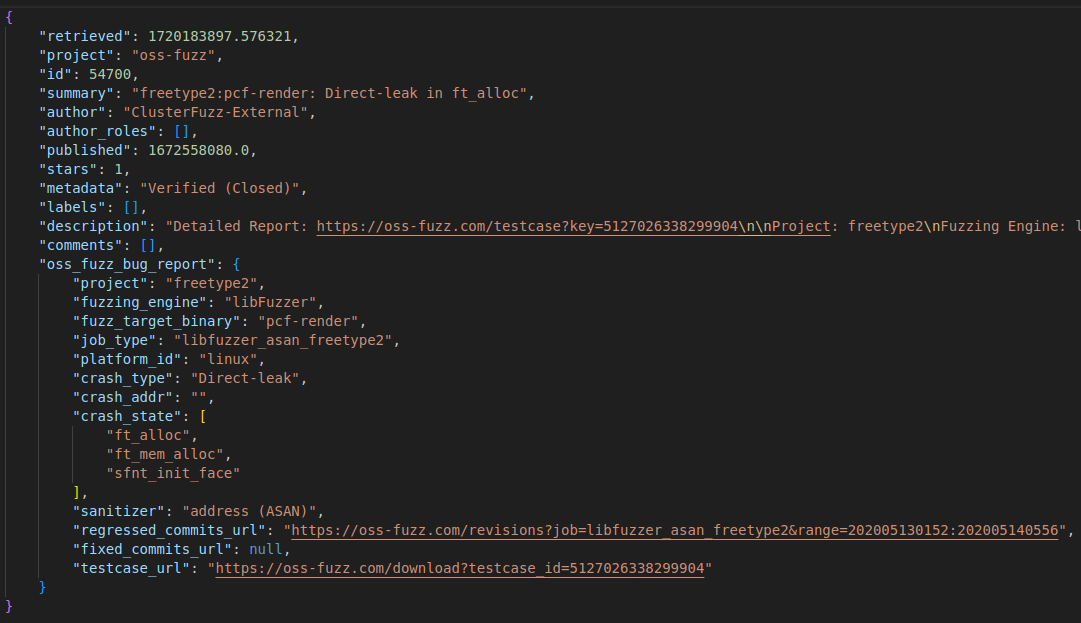
\includegraphics[width=0.66\paperwidth]{foto/json.png}}
\caption{Example of information collected from reports in JSON}
\label{fig:report}
\end{figure}
\ \\
The analysis was performed on all bugs between 2023-01-01 and 2024-06-31, for a total of 11743 collected reports.



\newpage
The second to last step was to analyze the previously obtained JSON files and make a list of the most bugged projects for each category.
\newline
To do this, I initially wrote a simple Python script that takes as input the JSON files and analyzes the information fields collected.
\newline
First, I checked the \textit{"metadata"} field for values like "WontFix", "Duplicate" or "Invalid": the first means that the developers themselves tagged that specific bug as non-relevant and will not be addressed in the future, the second refers to a report for a bug that has been already issued but triggered by a different testcase, while the last one means that the reported bug could not be reliably reproduced.
\newline
Then, I checked the \textit{"description"} field for manual reports, as they were not meaningful towards the final results. 
\newline
Assuming the report analyzed is valid and generated by ClusterFuzz, I retrieved the project name from the \textit{"oss\_fuzz\_bug\_report"} fields and used a dictionary key-value to keep track of the number of bugs reported for each project. 
\newline
\begin{figure}[h]
\centering
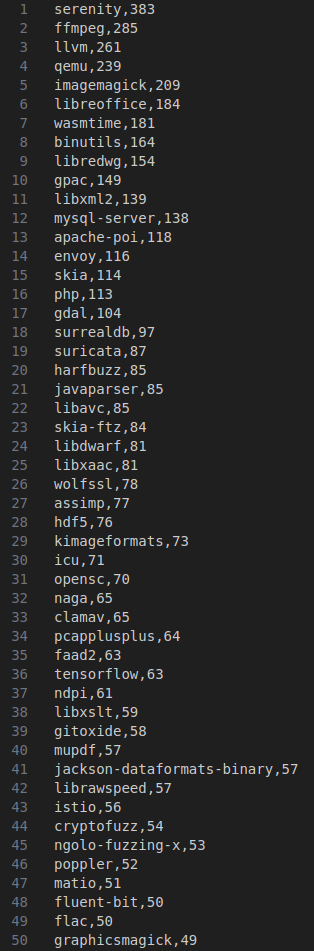
\includegraphics[scale=0.44]{foto/list.png}
\caption{Extract of the 50 most bugged projects}
\label{fig:list}
\end{figure}

\newpage
The last step was to analyze each project individually and determine which harness produced the highest number of reports.
\newline
Given the previous script, I extended it to take as input also a project name, so that the parsing of the JSON file focused only on reports for that particular project, and the dictionary key-value was now used to keep track of the number of bugs produced by each fuzzing target binary.
\ \\ \newline \newline
All this resulted in the following projects and harnesses being tested:
\begin{itemize}
  \item \textbf{All Sanitizers}
  \begin{itemize}
    \item binutils (fuzz\_objdump\_safe)
    \item harfbuzz (hb-subset-fuzzer)
    \item imagemagick (encoder\_heic\_fuzzer)
    \item libxml2 (valid)
    \item skia (skruntimeeffect)
  \end{itemize}
  \item \textbf{ASan + MSan}
  \begin{itemize}
    \item ghostscript (gs\_device\_pdfwrite\_fuzzer)
    \item libyang (lyd\_parse\_mem\_json)
    \item wasmedge (wasmedge-fuzztool)
    \item openjpeg (opj\_decompress\_fuzz\_J2K)
    \item myanmar-tools (zawgyi\_detector\_fuzz\_target)
  \end{itemize}
  \item \textbf{ASan + UBSan}
  \begin{itemize}
    \item cairo (svg-render-fuzzer)
    \item clamav (clamav\_dbload\_YARA\_fuzzer)
    \item freerdp (TestFuzzCoreClient)
    \item tarantool (luaL\_loadbuffer\_fuzzer)
    \item vlc (vlc-demux-dec-libfuzzer)
  \end{itemize}
  \item \textbf{ASan only}
  \begin{itemize}
    \item fwupd (uswid\_fuzzer)
    \item glslang (compile\_fuzzer)
    \item inchi (inchi\_input\_fuzzer)
    \item radare2 (ia\_fuzz)
    \item zeek (zeek-ftp-fuzzer)
  \end{itemize}
  \item \textbf{No Sanitizers}
  \begin{itemize}
    \item fluent-bit (flb-it-fuzz-cmetric\_decode\_fuzz\_OSSFUZZ)
    \item gpac (fuzz\_probe\_analyze)
    \item libdwarf (fuzz\_debug\_str)
    \item libredwg (llvmfuzz)
    \item serenity (FuzzJs)
  \end{itemize}
\end{itemize}








\newpage
\subsection{Testing with OSS-Fuzz}
The OSS-Fuzz repository contains several tools to build and test the available projects, as well as debugging and reproduction scripts.
\newline
Most of the tools used in this work are provided by the "helper.py" script, which I used to download a project's Docker image, build the fuzzers as well and download the public corpora made available by the developers.
\newline \newline
The commands used are:
\begin{verbatim}
$ python3 helper.py pull_images 

$ python3 helper.py build_image {project_name}

$ python3 helper.py build_fuzzers {project_name}
    --sanitizer={address(default),memory,undefined,none} 
        --engine={libfuzzer(default),afl, honggfuzz, centipede}
        
$ python3 helper.py download_corpora 
    --project={project_name} --fuzz-target={harness_name}
\end{verbatim}
\ \\
The \verb|pull_images| argument connects to OSS-Fuzz's Google Bucket to download and update all the Docker "base images" on your local machine, which are used by all projects as the base image to create their respective testing environment.
\newline \newline
The \verb|build_image| argument takes as input the name of a project and builds its Dockerfile, creating a new image on your local machine that will be later used to perform fuzzing. During this process, all dependencies and resources needed to correctly compile the fuzzers are downloaded and installed, including the main \textit{build.sh} script. It was used in conjunction with daily \verb|git pull| on the OSS-Fuzz repository, to make sure that I was always building the latest version. 
\newline \newline
The \verb|build_fuzzers| argument takes as input the name of a project and a list of possible sanitizers and fuzzing engines to be used during the compilation of the fuzz targets. Although this command accepts only one sanitizer and fuzzing engine at a time, it's possible to mix them by acting on some environment variables provided by the base images. Finally, this script acts as a "wrapper" for a much more complex Docker command, that creates the project's Docker image using some specific environment variables and invokes the execution of the \textit{build.sh} script.
\newline \newline
The \verb|download_corpora| argument takes as input a project name and a fuzz target, it then connects to the project's Google Bucket and downloads the latest public corpus for the provided fuzz target.
\newline \newline \newline
After executing these commands, three new directories are created.
\newline
The "out" directory contains the project's directory where all the built files are saved, including libraries, fuzz targets and other files created by the selected fuzzer.
\newline
The "work" directory acts as a temporary location to store intermediate files during the building process, it may also we used to store the fuzzing session results.
\newline
The "corpus" directory contains the downloaded corpora stored as zip files.



\newpage
To prepare the tests, I was tasked with building the chosen harnesses using all possible values for sanitizers, meaning that each project was compiled 4 times: with ASan only, with MSan only, with UBSan only and without any sanitizer.
\newline
Moreover, all projects were built using AFL as fuzzing engine, because (perché abbiamo usato AFL ???) 
\newline \newline
The tests were performed inside each project's Docker image, created and configured using the following command:
\begin{verbatim}
    $ docker run --rm --privileged --platform linux/amd64 
        -v /oss-fuzz/build/out/{project_name}/:/out/  
        -v /home/zio-saba/Scrivania/TESI/results/:/results/ 
        -it  gcr.io/oss-fuzz/{project_name} /bin/bash
\end{verbatim}
\ \\
This is a shorter and modified version of the command invoked by the \verb|build_fuzzer| wrapper.
\newline \newline
The first few parameters are needed to create a privileged instance of Docker and specify the running platform on which the fuzz targets will be tested.
\newline \newline
The arguments starting with \verb|-v| are used to create a shared directory in the Docker container, more specifically by linking a local directory to a virtual one created inside the container. This was needed to make sure that I could access the fuzzers, built in a Docker container and then locally stored on my machine, from inside the Docker container used for the tests.
\newline \newline
The last line invokes the project image to load as well as making it interactive by spawning a \verb|/bin/bash| process.




\newpage
When i had problems, i Didi this:
\begin{verbatim}
    $ docker run --rm --privileged --platform linux/amd64 
        -e PROJECT_NAME={project_name} -e HELPER=True 
        -e FUZZING_LANGUAGE=c++ 
        -e FUZZING_ENGINE=afl 
        -e SANITIZER={address,memory,undefined,none} 
        -v /oss-fuzz/build/out/{project_name}/:/out/
        -v /oss-fuzz/build/work/{project_name}/:/work/
        -it  gcr.io/oss-fuzz/{project_name} /bin/bash
\end{verbatim}






\ \\ \newline \newline
Explain how projects were built and how to retrieve the corpus....
\newline \newline
Explain how tests were automated and their duration...
\newline \newline
Explain how you can build a project on your own machine...
\newline \newline
Explain the Dockerfile to build the project's image...
\newline \newline
Explain the build.sh to build the harnesses...
\newline \newline
Explain the commands from /infra/helper.py...
\subsubsection{??? Un singolo esempio di test mostrato per intero ???}

\newpage
\section{FuzzBench}
\subsection{Selecting the projects}
Explain the selection process and the chosen test set...
\newline \newline
Explain how the experiment\_project.yaml analysis was performed...
\newline \newline
Explain how crashes and corpus were obtained through scraping...
\newline \newline
\subsection{Testing with FuzzBench}
Explain how projects were built....
\newline \newline
Explain how tests were automated and their duration...
\subsubsection{??? Un singolo esempio di test mostrato per intero ???}


\newpage
When i testef fuzzbench and had to build using ASan + UBSan, i Didi this:
\begin{verbatim}
    $ docker run --rm --privileged --platform linux/amd64 
        -e PROJECT_NAME={project_name} -e HELPER=True 
        -e FUZZING_LANGUAGE=c++ -e FUZZING_ENGINE=afl 
        -e SANITIZER=address 
        -e SANITIZER_FLAGS_address="
            -fsanitize=address,array-bounds,bool,builtin,enum,
                integer-divide-by-zero,null,object-size,return,
                returns-nonnull-attribute,shift,
                signed-integer-overflow,unsigned-integer-overflow,
                unreachable,vla-bound,vptr
            -fno-sanitize-recover=array-bounds,bool,builtin,enum,
                integer-divide-by-zero,null,object-size,return,
                returns-nonnull-attribute,shift,
                signed-integer-overflow,unreachable,
                vla-bound,vptr 
            -fsanitize-address-use-after-scope" 
        -v /oss-fuzz/build/out/{project_name}/:/out/  
        -v /oss-fuzz/build/work/{project_name}/:/work/
        -it  gcr.io/oss-fuzz/{project_name} /bin/bash
\end{verbatim}


\newpage
\chapter{Results}
\ \\
Explain how the results were analyzed...
\newline \newline
Briefly explain the python scripts used to retrieve the results...



\newpage
\section{OSS-Fuzz: No Sanitizers}
Show table
\newline \newline
Discuss results...

\newpage
\section{OSS-Fuzz: ASan Only}
Show table
\newline \newline
Discuss results...

\newpage
\section{OSS-Fuzz: ASan + MSan}
Show table
\newline \newline
Discuss results...

\newpage
\section{OSS-Fuzz: ASan + UBSan}
Show table
\newline \newline
Discuss results...

\newpage
\section{OSS-Fuzz: All Sanitizers}
Show table
\newline \newline
Discuss results...

\newpage
\section{Case study 1: ???}


\newpage
\section{Case study 2: ???}


\newpage
\section{FuzzBench}


\newpage
\section{Case study 1: ???}


\newpage
\section{Case study 2: ???}


\newpage
\section{About the results obtained}
Discuss the overall results, what was expected and what was unexpected...
\newline \newline
Discuss the importance of such results, what can be inferred...
\newline \newline
??? Discuss about the reports  where???












\chapter{Conclusions (final considerations???, future works???)}
\ \\
Briefly recap what was done, the results obtained and their importance...
\newline \newline
Talk about what can be inferred from this study, what this study highlighted and why it is important...
\newline \newline
Discuss the reports and the developers' answers, including some considerations about their responses...
\newline \newline
Talk about what could/should be done to improve the situation...
\newline \newline
Future works???





\backmatter
\phantomsection
\begin{thebibliography}{0}

\bibitem{ref:AFL}
\textit{American Fuzzy Lop}
\newline
\url{https://lcamtuf.coredump.cx/afl/}

\bibitem{ref:shellshock}
\textit{"The Shellshock Incident Explained"}
\newline
\url{https://www.exploit-db.com/docs/english/48112-the-shellshock-attack-%5Bpaper%5D.pdf?ref=benheater.com}

\bibitem{ref:heartbleed}
\textit{"The Heartbleed Bug Explained"}
\newline
\url{https://heartbleed.com/}

\bibitem{ref:doc-ossfuzz}
\textit{The OSS-Fuzz Project Documentation}
\newline
\url{https://google.github.io/oss-fuzz/}

\bibitem{ref:doc-fuzzbench}
\textit{The FuzzBench Project Documentation}
\newline
\url{https://google.github.io/fuzzbench/}

\bibitem{ref:san_repo}
\textit{Google Sanitizers' GitHub Repository}
\newline
\url{https://github.com/google/sanitizers}

\bibitem{ref:asan_paper}
Konstantin Serebryany, Derek Bruening, Alexander Potapenko and Dmitry Vyukov, "\textit{AddressSanitizer: A Fast Address Sanity Checker}", Proceedings of the 2012 USENIX conference on Annual Technical Conference (USENIX ATC 12), June 2012
\newline
\url{https://www.usenix.org/system/files/conference/atc12/atc12-final39.pdf}

\bibitem{ref:msan_paper}
Evgeniy Stepanov and Konstantin Serebryany, "\textit{MemorySanitizer: fast detector of uninitialized memory use in C++}", Proceedings of the 13th Annual IEEE/ACM International Symposium on Code Generation and Optimization (ACM CGO '15), February 2012
\newline
\url{https://static.googleusercontent.com/media/research.google.com/it//pubs/archive/43308.pdf}

\bibitem{ref:asan_docs}
\textit{Address Sanitizer Documentation}
\newline
\url{https://clang.llvm.org/docs/AddressSanitizer.html}

\bibitem{ref:msan_docs}
\textit{Memory Sanitizer Documentation}
\newline
\url{https://clang.llvm.org/docs/MemorySanitizer.html}

\bibitem{ref:ubsan_docs}
\textit{Undefined Behavior Sanitizer Documentation}
\newline
\url{https://clang.llvm.org/docs/UndefinedBehaviorSanitizer.html}

\bibitem{ref:afl_docs}
\textit{LibAFL Fuzzing Library}
\newline
\url{https://aflplus.plus/libafl-book/libafl.html}

\bibitem{ref:osd}
\textit{"Open-Source License" Definition}
\newline
\url{https://opensource.org/osd}

\bibitem{ref:google_oss}
\textit{Google Open Source Project}
\newline
\url{https://opensource.google/}

\bibitem{ref:ossfuzz_docs}
\textit{OSS-Fuzz Project Documentation}
\newline
\url{https://google.github.io/oss-fuzz/}

\bibitem{ref:clusterfuzz_docs}
\textit{ClusterFuzz Project Documentation}
\newline
\url{https://google.github.io/clusterfuzz/}

\bibitem{ref:fuzzbench_docs}
\textit{FuzzBench Project Documentation}
\newline
\url{https://google.github.io/fuzzbench/}

\bibitem{ref:libfuzzer_docs}
\textit{LibFuzzer Documentation}
\newline
\url{https://llvm.org/docs/LibFuzzer.html}

\bibitem{ref:ossfuzz_bugtracker}
\textit{OSS-Fuzz Issue Tracker}
\newline
\url{https://issues.oss-fuzz.com/issues}

\bibitem{ref:bug_disclosure}
\textit{Google Project Zero: Bug Disclosure Guidelines}
\newline
\url{https://googleprojectzero.blogspot.com/2015/02/feedback-and-data-driven-updates-to.html}

\bibitem{ref:valgrind}
\textit{Valgrind Website}
\newline
\url{https://valgrind.org/}

\bibitem{ref:score}
\textit{Open-Source Project Criticality Score}
\newline
\url{https://github.com/ossf/criticality_score}

\bibitem{ref:scraper}
\textit{Monorail Scraper GitHub Repository}
\newline
\url{https://github.com/zhenyudg/monorail-scraper}

\bibitem{ref:driver}
\textit{GoogleDriver for Google Chrome}
\newline
\url{https://developer.chrome.com/docs/chromedriver?hl=it}

\bibitem{ref:driver_standard}
\textit{W3C WebDriver Documentation}
\newline
\url{https://w3c.github.io/webdriver/}

\end{thebibliography}




\end{document}